\chapter{Implementazione su LUNES}

\begin{figure}[H]
    \centering
    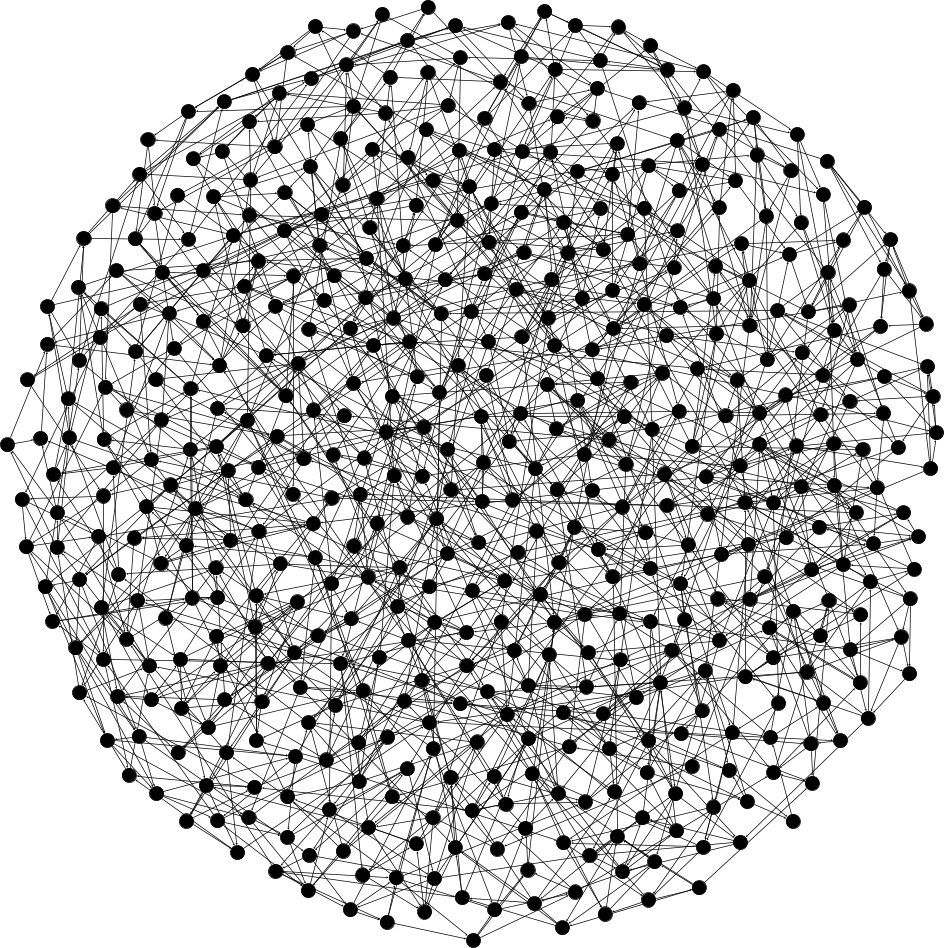
\includegraphics[width=0.6\textwidth]{images/network-500.png}
    \caption{Visualizzazione di una rete di esempio con $500$ nodi e $10000$ vertici generata con \textit{igraph}.}
\end{figure}
L'implementazione dei test con i vari scenari di attacco è stata effettuata in \textit{C} utilizzando le API messe a disposizione da \textit{GAIA} tramite \textit{LUNES}.\newline
\textit{LUNES} permette di costruire una piattaforma ed eventi molto performante capace di far interagire le varie \textit{Simulated Entities} utilizzando anche il vincolo del tempo. Il simulatore, infatti, essendo \textit{time-stepped} permette di utilizzare la componente \textit{tempo} come parte integrante della simulazione. Il tempo all'interno della simulazione non rispecchia quello del mondo reale e permette di valutare dei processi molto lunghi come composto di singoli step. Ad esempio l'operazione di \textit{mining} dei nodi non può essere replicata rispecchiando le tempistiche reali ma conoscendo alcuni parametri è possibile costruirne la funzione di probabilità ed applicarla alla simulazione.\newline
Il simulatore è inizialmente si occupa di inizializzare i \textit{peer} ed i collegamenti sulla base di un grafo generato tramite la libreria \href{https://igraph.org/}{\textit{igraph}}. Con la creazione della rete vengono inizializzate anche le strutture dati, usate dai \textit{peer}, per il salvataggio di dati, scambio di informazioni, informazioni sul proprio stato e della rete.\newline
La gestione delle interazioni tra i vari \textit{peer} è gestita come una macchina a stati finita che reagisce ai vari eventi in arrivo ai nodi. Ogni evento è caratterizzato da una singola azione che il nodo può compiere e quindi questa progettazione modulare risulta essere molto estensibile: per ogni nuova azione aggiuntiva è sufficiente generare la gestione per il singolo evento.\newline
Utilizzando il \textit{SIMA} di \textit{ARTÌS} e \textit{GAIA} non è necessario progettare od implementare i meccanismi di comunicazione e \textit{load balancing} che la progettazione del progetto prevede. In aggiunta \textit{LUNES} fornisce alcune implementazioni dei maggiori algoritmi di \textit{gossip} [\ref{appendix:gossip}] come \texttt{broadcast}, \texttt{broadcast probabilistico} e \texttt{broadcast dipendente dal grado}. Non è presente però l'algoritmo \texttt{Dandelion} utilizzato nella reale implementazione dei client per Bitcoin. Questa mancanza non risulta essere bloccante in quanto è dimostrato\cite{gdalunes} che le implementazioni degli algoritmi di \textit{gossip} messi a disposizione da \textit{LUNES} consentono di raggiungere il $100\%$ di copertura della rete con un ridotto volume di \textit{overhead}.

\textit{Dandelion} non è stato progettato per garantire sicurezza aggiuntiva ma per ovviare al problema della parziale anonimità di Bitcoin; risulta, quindi, non necessario ai fini del lavoro di tesi.

\section{Dimensionamento}
Il numero di \textit{peer} totali stimato appartenenti alla rete Bitcoin è di circa $10400$ \cite{bitnodes}\footnote{Bitnodes è stato sviluppato per stimare la dimensione della rete Bitcoin cercando gli host raggiungibili. La metodologia utilizzata prevede l'invio di messaggi \texttt{getaddr} ricorsivamente per scoprire tutti noti della rete partendo da un insieme di peer conosciuti. Il \textit{crawler} è stato implementato in Python ed è disponibile con licenza \textit{MIT} su GitHub}) ma non è possibile effettuare una stima esatta data la dinamicità e vastità della rete. I nodi attivi non costituiscono dei nodi \textit{miner} in quanto non tutti i peer devono partecipare attivamente al processo di creazione dei blocchi ma contribuiscono alla ricezione, validazione e broadcast delle transazioni e dei blocchi mantenendo sempre aggiornata la blockchain. I \textit{miner}, infatti, sono stimati essere circa $1$ milione ma quasi la totalità si affida ad un \textit{pool} per distribuire il carico di lavoro ed avere maggior probabilità di guadagno dalle transazioni \textit{coinbase} o non sono dei \textit{full node}.\newline
Ai fini di questo progetto di tesi non vengono considerati i singoli miner presenti all'interno dei \textit{pool} in quanto i vari scenari di attacco non sono eseguibili. Un \textit{miner}, ad esempio, con il $51\%$ di potenza di calcolo globale aumenterebbe le probabilità di guadagno del \textit{pool} e degli altri utilizzatori; un \textit{double spending} risulterebbe impossibile in quanto il \textit{pool} agisce come intermediario tra i \textit{miner} e la rete.\newline
Sono, quindi, considerati i \textit{miner} singoli e i \textit{pool} nella loro interezza come dei \texit{full node}: ogni nodo della rete partecipa alla trasmissione dei messaggi ed al mantenimento della propria blockchain.
\begin{figure}[H]
    \centering
    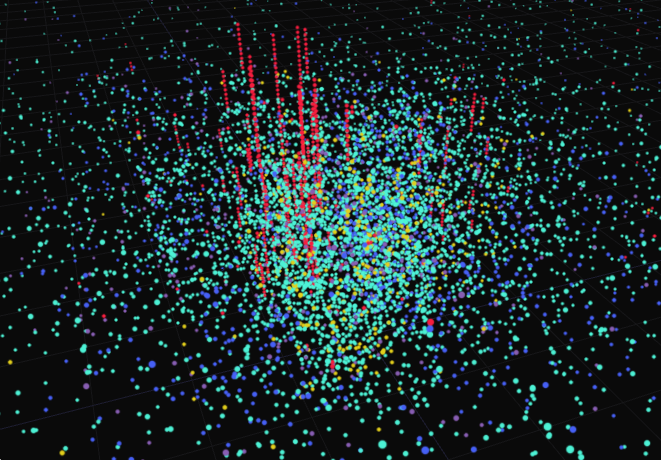
\includegraphics[width=0.8\textwidth]{images/bitnodes.png}
    \caption{Visualizzazione di una porzione di nodi attivi elaborati e classificati da \textit{Bitnodes} in base all'ultimo rilevamento online (i colori rappresentano il grado di sincronizzazione).}
    \source{Bitnodes}
\end{figure}

\section{Mining}
La simulazione del processo di \textit{mining} dei nodi è modellata in modo tale che rispetti difficoltà ed andamento paragonabili a quelli reali ma senza l'esigenza computazione e temporale richiesta dal protocollo Bitcoin. I blocchi sono pubblicati e creati in un intervallo di tempo di circa $10$ minuti. Per ovviare al problema dell'aumento dell'\textit{hashrate} dell'intera rete, Bitcoin implementa un meccanismo di \textit{difficoltà} secondo il quale ogni $2016$ blocchi la probabilità di trovare il \textit{nonce} corretto varia proporzionalmente alla potenza di calcolo dell'intera rete.\newline
Il valore della \textit{difficoltà} varia in base all'equazione \ref{eq:difficulty}; di conseguenza è possibile calcolare la probabilità di calcolo del \textit{nonce} corretto in base ad un tempo $T$ (minuti) è:
\begin{equation}
    P = \exp^{-T/10}
\end{equation}
Ai fini della simulazione è interessante calcolare la probabilità di calcolo di un blocco data una percentuale di hashrate in un dato tempo $T$. Ogni \textit{miner} $m$ possiede una frazione $h$ della potenza di calcolo totale $H$; tramite la distribuzione di Poisson, quindi, è possibile sapere quale è la probabilità che un nodo trovi il blocco in un dato tempo $T$:
\begin{equation}\label{eq:mining}
    P_m = (h * H / 100) * T / (2^{32} * D)
\end{equation}
Dove $D$ è il valore della \textit{difficoltà} allo stato attuale della rete con un \textit{hashrate} totale di $H$ espresso in $G/s$ o $G/min$ (di conseguenza $T$ è espresso in secondi o minuti). Ad esempio utilizzando un \textit{ASIC} con potenza di calcolo di $13$ TeraHash al secondo la probabilità di calcolare un blocco in $10$ minuti è del $0.00000027295900726337\%$ (dati gli attuali valori di $H$ e $D$, Novembre 2018).\newline
Conoscendo la distribuzione della probabilità nel tempo per ogni nodo è possibile evitare ogni tipo di attività di calcolo del \textit{nonce} tramite \textit{Hashcash} e facilitarne la simulazione: ad ogni step i \textit{miner} hanno una possibilità di calcolare e pubblicare un blocco data dall'equazione \ref{eq:mining}.
\begin{figure}[H]
    \centering
    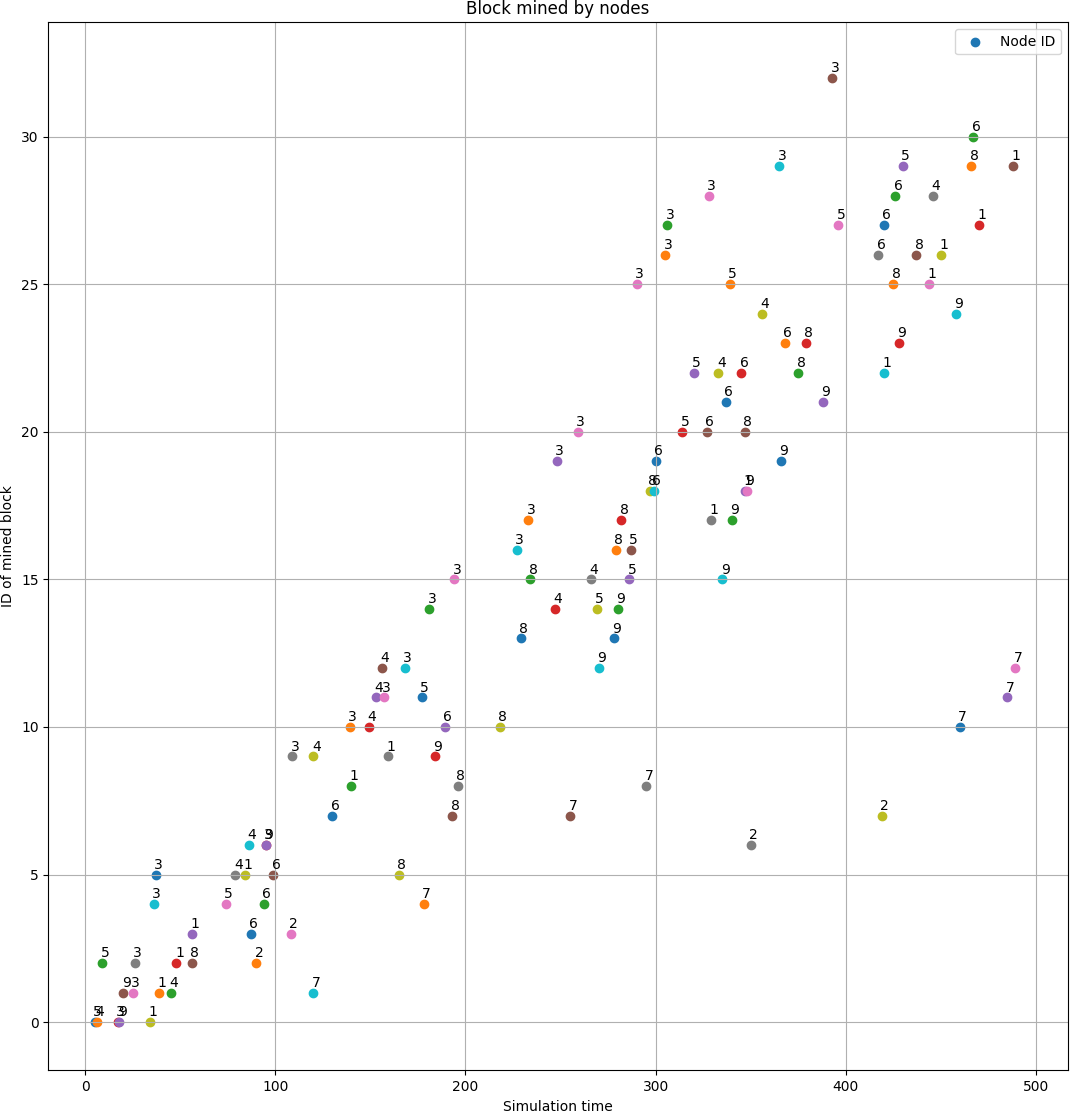
\includegraphics[width=\textwidth]{images/blockmined.png}
    \caption{Visualizzazione dei blocchi creati da ogni nodo nel corso di una simulazione di test.}
\end{figure}

\section{Messaggi}
Ogni nodo della rete può inviare o ricevere messaggi in accordo con la 



% NeoTex: mainfile=main.tex:
